\documentclass[aps,prd,10pt,twocolumn,superscriptaddress,showpacs]{revtex4-1}
\usepackage{titlesec}
\usepackage{hyperref}
\usepackage{graphicx}
\usepackage{amsfonts,amsmath,amssymb,bm,bbm}
\usepackage{color}
\usepackage{caption}
\usepackage{subcaption}

\hypersetup{
    pdfnewwindow=true,      % links in new window
    colorlinks=true,       % false: boxed links; true: colored links
    linkcolor=blue,          % color of internal links
    citecolor=blue,        % color of links to bibliography
    filecolor=blue,      % color of file links
    urlcolor=blue        % color of external links
}

\titleformat{\section}[runin]
  {\normalfont\bfseries}{\thesection}{1em}{}[:]
\titlespacing*{\section}{0cm}{2em}{1em}
\titleformat{\subsection}[runin]
  {\normalfont\itshape}{\thesubsection}{1em}{}[:]
\titlespacing*{\subsection}{1cm}{2em}{1em}

\titleformat{\section}[runin]
  {\normalfont\bfseries}{\thesection}{1em}{}[:]
\titlespacing*{\section}{0cm}{2em}{1em}
\titleformat{\subsection}[runin]
  {\normalfont\itshape}{\thesubsection}{1em}{}[:]
\titlespacing*{\subsection}{1cm}{2em}{1em}

\newcommand{\bvec}[1]{\mathbf{#1}}
\newcommand{\units}[1]{\,\mathrm{#1}}
\newcommand{\comments}[1]{}

\graphicspath{{../img/}}

\begin{document}

\title{The Doppler effect on indirect detection of dark matter}
\author{Devon Powell}
\email{dmpowel1@stanford.edu}
\author{Ranjan Laha}
\email{rlaha@stanford.edu}
\author{Tom Abel}
%\email{tabel@stanford.edu}
\affiliation{Kavli Institute for Particle Astrophysics and Cosmology (KIPAC),
	\\ Department of Physics, Stanford University, Stanford, CA 94305, USA}
\affiliation{SLAC National Accelerator Laboratory, Menlo Park, CA 94025, USA}
\date{\today}

\begin{abstract}
\cite{speckhard2016}
\end{abstract}

%\pacs{95.35.+d, 13.35.Hb, 14.60.St, 14.60.Pq}
% 95.35.+d Dark matter
% 13.35.Hb Decays of heavy neutrinos
% 14.60.St Non-standard-model neutrinos, right-handed neutrinos, etc.
% 14.60.Pq Neutrino mass and mixing 

\maketitle


% % % % % % % % % % % INTRODUCTION % % % % % % % % % % % % % % % % % % % % % %
\section{Introduction}
\label{sec:Introduction}

The search for the particle properties of dark matter is one of the most important research avenues\,\cite{Jungman:1995df,Bertone:2004pz,Strigari:2013iaa}.  The ``weak" interactions experienced by the dark matter particle complicates these searches.  Despite decades of multi-pronged searches, we have not yet identified the dark matter particle\,\cite{Bertone:2016nfn}.  One of the most important ways to search for dark matter particles is indirect detection\,\cite{Klasen:2015uma}.

Many anomalous signals have been interpreted as arising from dark matter interactions\,\cite{Loewenstein:2009cm,Prokhorov:2010us,Weniger:2012tx,Abazajian:2014hsa,Lee:2015fea,Bartels:2015aea,Bulbul:2014sua,Boyarsky:2014jta,Urban:2014yda}.  Astrophysical sources such as pulsars or atomic lines are diverse enough to mimic a dark matter signal\,\cite{O'Leary:2015gfa,Brandt:2015ula,O'Leary:2016osi,Gu:2015gqm,Phillips:2015wla,Shah:2016efh}.  The separation of signal and background is difficult since one needs to model these in the same data set.  Taking lessons from all these misadventures, it is prudent to ask for new methods to cleanly separate the signal and background.  This is especially important since there are many viable dark matter candidates which can only be detected via astrophysical observations.  

Distinct kinematic signatures arising from dark matter annihilation or decay are used to separate the dark matter signal from background.  These signatures include monochromatic photons arising from dark matter annihilation or decay.  Past experiences have shown that it is not reliable to only depend on this kinematic end point signature for the identification of a dark matter signal.  Additional checks are required to completely confirm a dark matter signal.  

In order to better characterize a dark matter signal, Ref.\,\cite{speckhard2016} utilized the superb energy resolution, $\sim \mathcal{O}$(0.1\%), of Hitomi (previously known as Astro-H) to find a new signature --- dark matter velocity spectroscopy.  Solar motion around the Galaxy produces a distinct longitudinal dependence in the dark matter signal, a signature of Doppler effect.  This new signature is model independent and applicable to any dark matter signal containing a sharp feature.  It is unlikely that baryonic phenomenon can produce such a distinct signature\,\cite{speckhard2016}.

Given the importance of dark matter particle searches, it is important to characterize any new model independent signature in detail.  While Hitomi had a narrow field of view, it is important to confirm if dark matter velocity spectroscopy can also be performed by a high energy resolution instrument with a wide field of view.  We perform such a study in this work using dark matter only simulations from Ref.\,\cite{mao2015}.  As an example of the dark matter signal, we consider the 3.5 keV line\,\cite{Bulbul:2014sua,Boyarsky:2014jta}.  The status of the 3.5 keV line is controversial\,\cite{Iakubovskyi:2015wma,Jeltema:2015mee,Ruchayskiy:2015onc,Bulbul:2016yop,Aharonian:2016gzq,Hofmann:2016urz,Arguelles:2016uwb,Conlon:2016lxl,Neronov:2016wdd,Perez:2016tcq}.  The malfunctioning of the Hitomi satellite did not permit an observation to conclusively test this signal.  We use future Micro-X observations\,\cite{Figueroa-Feliciano:2015gwa} to demonstrate our technique.  It is expected that Micro-X will have an energy resolution of 3 eV at 3.5 keV\,\cite{Figueroa-Feliciano:2015gwa}, a high enough energy resolution to permit dark matter velocity spectroscopy\,\cite{speckhard2016}.  We emphasize that we are using this 3.5 keV signal as a proxy, and that the underlying physics of dark matter velocity spectroscopy is model independent. 

There have been many works in which velocity spectroscopy was used to understand baryonic astrophysical emission\,\cite{Dame:2000sp,Diehl:2006cf,Kalberla:2008uu,Kretschmer:2013naa}.  Ref.\,\cite{speckhard2016} first applied this technique analytically to dark matter.  In this work, we analyze for the {\it first} time dark matter velocity spectroscopy using realistic dark matter simulations 

Any telescope with $\mathcal{O}$(0.1 \%) energy resolution can perform dark matter velocity spectroscopy.  An improvement in the energy resolution is the natural step in the evolution of telescope instrumentation.  This improvement will help in disentangling the dark matter signal from background, and improve our knowledge of the astronomical sources.  For certain wavelengths, it is already known how to build a detector with $\mathcal{O}$(0.1\%) energy resolution, such as INTEGRAL/ SPI\,\cite{2003AA} and Hitomi.  Near future instruments like Micro-X\,\cite{Figueroa-Feliciano:2015gwa} and ATHENA X-IFU\,\cite{Barret:2016ett} will also have $\mathcal{O}$(0.1\%) energy resolution.

% % % % % % % % % % % METHODS % % % % % % % % % % % % % % % % % % % % % %
\section{Methods}
\subsection{Theory}
\label{sec:theory}

In this subsection, we outline the theoretical insights leading to dark matter velocity spectroscopy\,\cite{speckhard2016}.  The discussion is tailored for a wide field of view instrument like Micro-X.

For instruments with an energy resolution, $\Delta E/E$ $\gg$ $\mathcal{O} (0.1\%)$, the differential flux of photons originating from dark matter decay in the Milky Way halo is given by\,\cite{Figueroa-Feliciano:2015gwa}:
\begin{eqnarray}
\dfrac{d^2 \mathcal{F}}{d\Omega \, dE} =  \dfrac{\Gamma}{4\pi \, m_s} \, \dfrac{dN(E)}{dE} \, \int _0 ^{s_{\rm max}}  \, ds \, \rho[r(s, \Omega)]  \,.
\label{eq:double differential for the flux}
\end{eqnarray}
Here $\mathcal{F}$ denotes the flux in cm$^{-2}$ s$^{-1}$, $\Omega$ denotes the solid angle in sr, $E$ denotes the energy of the photon in keV, and $\Gamma$ denotes the decay rate (in s$^{-1}$) of the dark matter particle of mass $m_s$ (in keV).  The dark matter density (in keV cm$^{-3}$) profile is denoted by $\rho(r)$, and the photon spectrum (in keV$^{-1}$) is denoted by $dN(E)/dE$.  The line of sight distance, $s$, varies from 0 to $s_{\rm max}$, where the maximum value of the line of sight distance, $s_{\rm max}$, corresponds to the virial radius of the Milky Way halo.

In this work, we are concerned with sterile neutrino, $\nu_s$, decay to an active neutrino, $\nu_a$, and a photon, $\gamma$: $\nu_s \rightarrow \nu_a + \gamma$.  This implies that the photon energy $E = m_s/2$.  We concentrate on the detection of photons in this work, as the constraint from the detection of active neutrino is weak.

Observation by a telescope with $\sim$ $\mathcal{O}$(0.1\%) energy resolution modifies this above expression, Eqn.\,\ref{eq:double differential for the flux}, in two important and distinct ways.  First, the photon line is broadened due to the velocity dispersion of the dark matter particles in the Milky Way halo.  Second, the energy of the photon is shifted depending on the Doppler shifting of the line.  

We take into account the broadening of the line by convolving the $dN(E)/dE$ by a Gaussian of width $\sigma_E = (E/c) \sigma_{v_{\rm LOS}}$\,\cite{speckhard2016}.  Here $\sigma_{v_{\rm LOS}}$ corresponds to the line of sight velocity dispersion of dark matter.  The form of Gaussian arises since we consider a Maxwellian dark matter velocity distribution.  The line shape will change if we consider dark matter velocity distribution favored by recent hydrodynamical simulations\,\cite{Bozorgnia:2016ogo,Sloane:2016kyi,Kelso:2016qqj}, but we ignore the difference in this work.  

The broadened line shape can be written as 
\begin{eqnarray}
\dfrac{d \tilde{N} (E, r[s, \Omega])}{dE} &=& \int dE' \, \delta \left(E' - \dfrac{m_s}{2} \right) \nonumber\\
&\times& G(E - E', \sigma_{E'} (r[s, \Omega])) \, ,
\label{eq:formula for modified dNdE}
\end{eqnarray}
where the convolution function is a Gaussian as mentioned above.  The width of the Gaussian, $\sigma_E (r[s, \Omega])$ is calculated following Ref.\,\cite{speckhard2016}.

Since the solar velocity is nonrelativistic, we can use the usual formula for Doppler shift: $\Delta
E/E = - v_{\rm LOS}/c$.  Following Ref.\,\cite{speckhard2016}, we define $v_{\rm LOS} = (\langle
{\bf v}_\chi \rangle - {\bf v}_\odot) \cdot \hat{r}_{\rm LOS}$.  We assume $\langle {\bf v}_\chi
\rangle$ $\approx$ 0, and $v_\odot$ = 220 km s$^{-1}$.  In the coordinate system where the x-axis is
towards the Galactic Center, the direction of the Galactic rotation is in the y direction, and the
z-axis is the normal to the Galactic plane, we have ${\bf v}_\odot$ = $v_\odot \, \hat{y}$.  In this
reference frame, ${\bf v}_\odot \cdot \hat{r}_{\rm LOS}$ = $v_\odot y / |r_{\rm LOS}|$.  In terms of the Galactic longitude, $\ell$, and Galactic latitude, $b$, we have $y = r_{\rm LOS} \, {\rm sin} \, \ell \, {\rm cos} \, b$.  From this, we have $\Delta E/E = v_\odot \sin \ell\cos b$.

Taking these two effects into account, we can rewrite Eqn.\,\ref{eq:double differential for the flux} as 
\begin{eqnarray}
\dfrac{d^2 \mathcal{F} (\ell, b)}{d\Omega \, dE} &=&  \dfrac{\Gamma}{4\pi \, m_s} \, \int _0 ^{s_{\rm max}}  \, ds \, \rho[r(s, \Omega)] \nonumber\\
&\times& \dfrac{d \tilde{N}(E - \Delta E (\ell, b), r(s, \Omega))}{dE} \,.
\label{eq:double differential for the flux rewritten}
\end{eqnarray}
An important difference in the narrow field of view and wide field of view instruments is encapsulated in $\Delta E (\ell, b)$.  For Hitomi with a field of view of 9 arcmin$^2$, the maximum value of the line intensity approximately occurs at the ($\ell, \, b$) corresponding to the center of the field of view.  This is not true for a wide field of view instrument like Micro-X (20$^\circ$ radius field of view).  The maximum value of the line intensity depends on the density profile as is evident from Eqn.\,\ref{eq:double differential for the flux rewritten}.  

The shift in the central value of the energy of the widened line is shown by the argument $E - \Delta E (\ell, b)$.  Both the width of the line and the position of the central value of the line is determined by the position of the line and this is indicated by $r (s, \Omega)$ the argument of $d\tilde{N}/dE$.

\subsection{Analytic models}
\label{sec:simulations}

Here we describe the analytic models to which we compare the results of our N-body analysis. We
illustrate the difference between small- and large FOV instruments here, giving a model for each.

We begin with the model for the small FOV. The flux is given simply by the LOS integral, or
J-factor, divided by the solid angle. We take this approximation to mean that the flux is constant
over such a small FOV and can hence be approximated by a single line integral:
\begin{eqnarray}
\mathcal{F} (\ell, b) =  \frac{\Gamma}{4\pi \, m_s \Omega} \, \int _0 ^{s_{\rm max}}  \, ds \, \rho[r(s, \Omega)] 
\label{eq:lineflux}
\end{eqnarray}



\subsection{Simulations}
\label{sec:simulations}

Numerical simulations take into account many different processes which participate in dark matter halo formation.  Many signatures of these non linear processes are not taken into account in an analytical model of the dark matter halo.  It is thus important to validate any new signature of dark matter by using realistic simulations of galaxy formation.

We evaluate the potential of dark matter velocity spectroscopy using dark-matter-only N-body
simulations.  We study a suite of Milky Way analogues run using the L-GADGET cosmology code (a
descendant of GADGET-2\,\cite{springel2005}). These are dark-matter-only zoom-in simulations run by
Ref.\,\cite{mao2015} to study subhalo abundance. Their high resolution and multiple realizations
makes them suitable for our purposes as well. Each halo has $\mathcal{O}(10^7)$ high-resolution
particles with a particle mass $m_p=4.0 \times 10^5 M_{\odot}$ and total  mass
$M_{\mathrm{vir}}\simeq 10^{12} M_{\odot}$ (masses in physical units). Refer to \cite{mao2015} for
the full description of the simulation parameters.

We note that a $7\units{keV}$ sterile neutrino has a non-negligible free-streaming length 
and hence introduces a cutoff in
the matter power spectrum at a wavenumer $k_\mathrm{WDM} \simeq 10 \units{Mpc^{-1}\,h}$
\cite{ven2016}. This gives a corresponding mass scale cutoff of $M_\mathrm{WDM} \simeq 10^{10}
\units{M_\odot}$, or roughly $10^{-2}$ of the Milky Way halo mass. As we are interested in the main
halo itself, we do not concern ourself with the slight differences on smaller mass scales that may
arise due to our use of pure CDM simulations as a proxy for sterile neutrino dark matter. Ref. \cite{Lovell:2014lea}
discusses this in further detail and note that the flux maps for cold versus keV-mass dark matter
haloes differ by a few percent at most. While we focus on $m_s=7\units{keV}$ here,
one should view this study as a test model while noting that the velocity spectroscopy approach is
valid over a wide range of particle masses.

\begin{figure}[h!]
\centering
%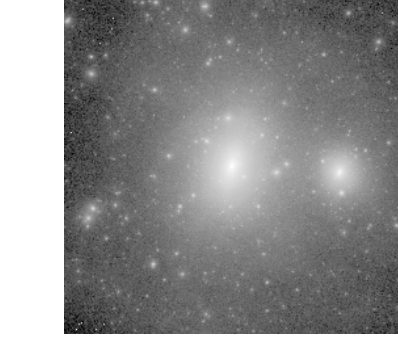
\includegraphics[width=0.9\columnwidth]{halo374.png}
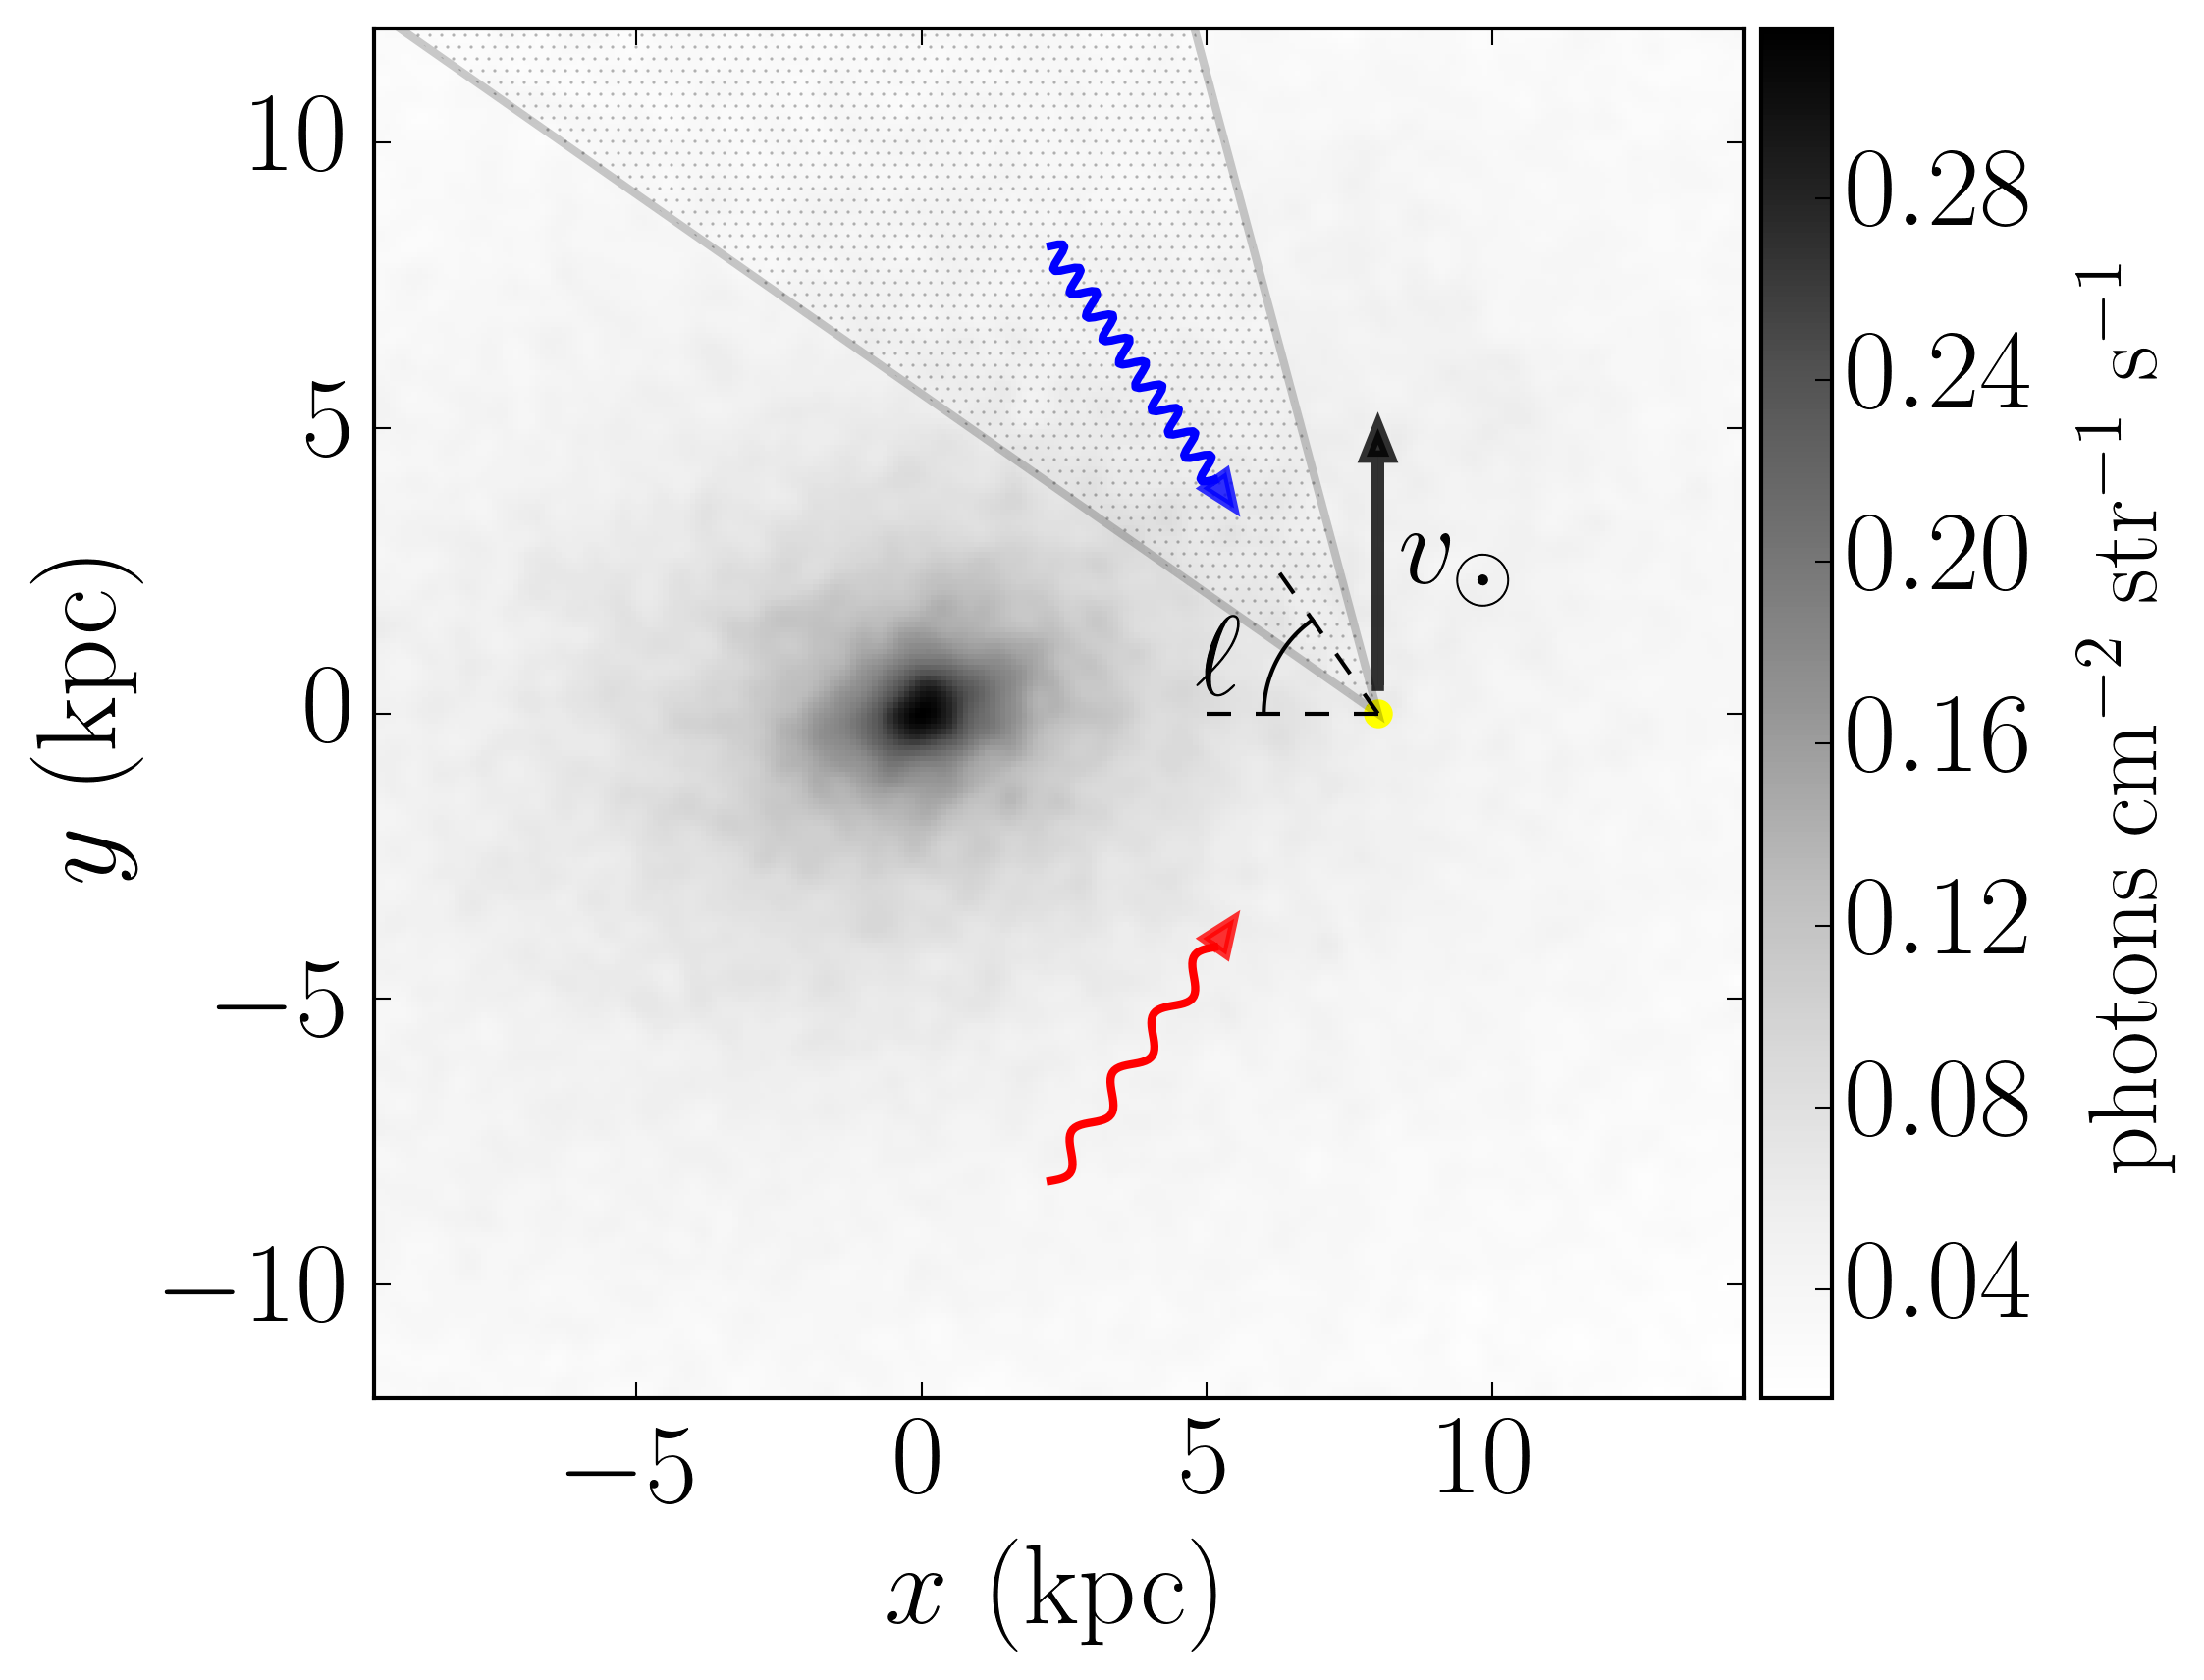
\includegraphics[width=0.99\columnwidth]{vspec_diagram.png}
\caption{The projected column density of Halo 374, the most spherical halo in the suite of
	simulations used here. The color scale is given in units of the photon flux at
the distance of the Sun, 8 kpc from the halo center. The diagram illustrates the basic principle of velocity
spectroscopy: X-ray photons due to sterile netrino decay are collected from within the field
of view (shaded triangle) at the Sun's position. The net blue- or redshift of observed photons 
is determined by the line of sight relative to the Sun's velocity. In this simple model, the energy
shift $\delta E/E=(v_\odot/c)\sin\ell$.}
\label{fig:halo374}
\end{figure}


Among the 46 halo realizations, we focus on one halo, Halo 374, (Figure\,\ref{fig:halo374}) in detail. This is the most spherically-symmetric halo, with principal axis ratios $b/a=0.86$ and $c/a=0.73$.  We choose this halo to facilitate the comparison of our results with a spherically symmetric generalized NFW profile of the halo.  Dark-matter-only simulations produce triaxial halos, but recent hydrodynamical simulations have shown that the inclusion of baryons tend to sphericalize a halo\,\cite{Debattista:2007yz,Bryan:2012mw,Bernal:2014mmt,Bernal:2016guq}.

Although hydrodynamical models are investigated by many groups, yet it is not known if all the baryonic processes are self consistently taken into account in these simulations.  To take into account these uncertainties, we will also show our results for halos which are less spherical compared to Halo 374.  The statistical significance of the result depends on the triaxiality of the halo.

\subsection{Velocity spectroscopy using simulations}
\label{sec:simulations}

In order to generalize the analytical methods presented in Sec.\,\ref{sec:theory} to a simulation
containing N-body particles, we simply convert the integration to a sum over the N-body particles.
This is similar in spirit to the ``sightline'' method employed by \cite{Lovell:2014lea} and the
velocity distribution function sampling of \cite{Mao:2012hf}.  We construct the full spectral
intensity seen by the detector directly from the N-body particles, incorporating Doppler shift and
velocity dispersion in a natural way.   

%The dark matter density field, $\rho({\bf{x}})$, in a position {\bf x} in an N-body simulation is effectively a sum of Dirac-$\delta$ functions:
%\begin{eqnarray}
%\rho({\bf{x}}) = \sum_p\, m_p \, \delta({\bf{x}} - {\bf{x}_p}) \, ,
%\end{eqnarray}
%where $\bf{x}_p$ and $m_p$ are the position and mass of particle $p$. 

The total flux can be found by integrating the differential flux in Eqn.\,\ref{eq:double differential for the flux} over the energy and solid angle.  Implementing this in an N-body simulation implies a summation over all of the particles, $p$, within the field of view, $\Omega$, and weighting by the inverse square of the scalar distance to the observer, $r^{-2}_p$:
\begin{eqnarray} 
\mathcal{F} = \frac{\Gamma}{4\pi \, m_s} \, \sum_{p \, \in \, \Omega} \, \frac{m_p}{r_p^{2}} \, ,
\end{eqnarray}

The differential flux in energy can also be calculated in a similar way:
\begin{eqnarray}
\label{eq:discrete}
\frac{d\mathcal{F}}{dE} = \frac{\Gamma}{4 \pi \, m_s}\, \sum_{p \, \in \, \Omega} \, \frac{m_p}{r_p^{2}} \, \frac{dN[E(1-v_p/c)]}{dE} \, ,
\end{eqnarray}
where $v_p$ is the velocity of particle $p$ projected along the line of sight to the observer.  By
considering the LOS velocity of each particle independently, we automatically capture the spectral
convolution introduced by the bulk velocity dispersion. 

We focus here on the special case where $dN/dE$ is a line due to sterile neutrino decay.  The
parameters of the sterile neutrino are those favored by the 3.5 keV line\,\cite{Bulbul:2014sua}.  In
this case, computing the observed spectrum is then as simple as building a flux-weighted histogram
of the line-of-sight velocities for all particles in the sampling cone. In practice we find
$d\mathcal{F}/dE$ to be roughly Gaussian, so we forgo binning and compute the line width directly
from the variance in LOS particle velocities. See Figure \ref{fig:dfde} for an illustration. 

\begin{figure}[h!]
\centering
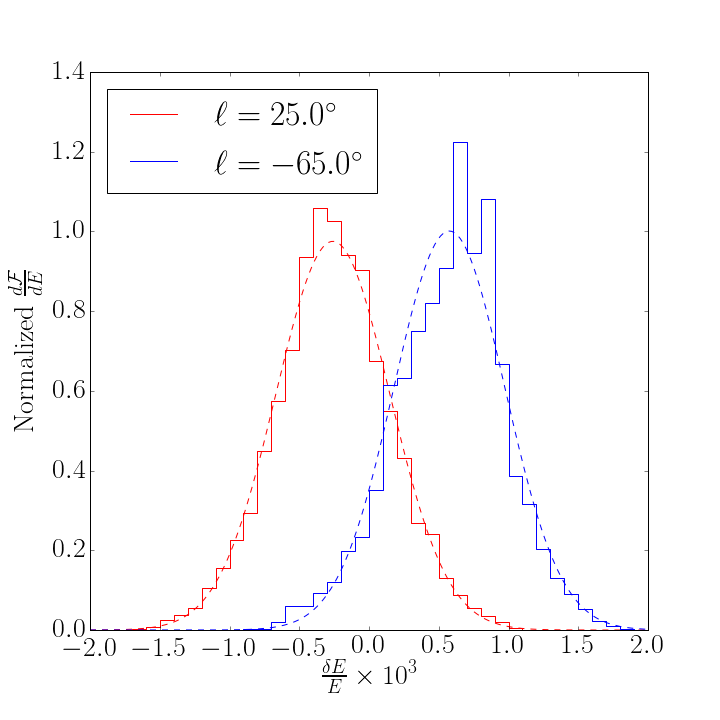
\includegraphics[width=1.0\columnwidth]{dnde_demo.png}
\caption{We plot the normalized $d\mathcal{F}/dE$ versus the fractional shift in the energy $\delta
E/E$ (the x-axis is multiplied by 1000 for clarity). The field of view is centered at $(\ell, b) =
(25^\circ, 25^\circ)$, and $(-65^\circ, 25^\circ)$.
	This compares the empirical histograms (solid) for the observed line spectrum
	$d\mathcal{F}/dE$ against their Gaussian models (dashed) as computed using \eqref{eq:simcenter} and \eqref{eq:simsigma}.
	The Gaussian approximation gives a good fit to the data and allows us to forgo binning in practice.}
\label{fig:dfde}
\end{figure}

The flux-weighted mean line-of-sight velocity for a field of view is 
\begin{eqnarray} 
	\langle v_{LOS} \rangle =\frac{1}{\mathcal{F}} \frac{\Gamma}{4\pi m_s} \sum_{p \, \in \, \Omega}
	\, \frac{m_p}{r_p^{2}} \, v_p
\label{eq:simcenter}
\end{eqnarray}
For non relativistic velocities, the mean Doppler shift (the observed shift in the energy of the line) is $\langle \delta E\rangle = (E/c)\langle v \rangle$.  We compute the width of the observed line $\sigma_E$ directly by finding the flux-weighted
variance of the line-of-sight velocities $v_p$:
\begin{equation} 
	\sigma_{v_{LOS}}^2 =\frac{1}{\mathcal{F}} \frac{\Gamma}{4\pi m_s} \sum_{p \, \in \, \Omega}
	\, \frac{m_p}{r_p^{2}} \left(v_p-\langle v_{LOS}\rangle\right)^2 
\label{eq:simsigma}
\end{equation}
The width of the Doppler-broadened line is then $\sigma_E = (E/c) \sigma_v$. 

We compare the line width and shift computed analytically and directly from simulations in Fig.\,\ref{fig:dfde} for two different field of views centered at $(\ell, b) \, = \, (25^\circ, 25^\circ)$ and $(-65^\circ, 25^\circ)$.  The analytical computation is shown by dashed line, whereas the solid line shows the lines computed directly from the simulations.  Good agreement is seen between these two different computations for this halo.

\subsection{Model observation by Micro-X}
\label{sec:microx}

The instrument that we focus on in this work is Micro-X\,\cite{Figueroa-Feliciano:2015gwa}.  It is a
direct successor to the XQC sounding rocket
experiment\,\cite{McCammon:2002gb,Boyarsky:2006hr,Crowder:2012ts}.  We follow the parameters of the
instrument near 3.5 keV as mentioned in\,\cite{Figueroa-Feliciano:2015gwa}: 20$^\circ$ radius field
of view, 1 cm$^2$ effective area, 96\% detector efficiency, 300 s exposure time, and 3 eV
energy resolution (FWHM). 

To minimize contamination by the Galactic plane, we focus on fields of view which are centered at $b = 25^\circ$ for various different Galactic longitudes, $\ell$.  This choice is a compromise between the decreasing signal strength away from the Galactic Center, and the more rapidly decreasing background away from the Galactic plane.  A typical sterile neutrino decay flux at $3.5$ keV from
the Milky Way halo at $b=25^\circ$ is $\mathcal{F}\sim 0.1$ photons\,cm$^{-2}$\,str$^{-1}$\,s$^{-1}$ 
for a signal count $N_s \sim 3-12$ photons, depending on $\ell$. 

We model the background $N_b$ using the cosmic X-ray background model of \cite{Ajello:2008xb}.  The
use of an alternative model\,\cite{Hickox:2005dz} for the cosmic X-ray background does not alter our
conclusions. For our analysis, we consider all photons observed in the range
$3.5\units{keV}\pm10.5\units{eV}$. This range contains all of the expected signal and captures
sufficient background counts for signal and background to be differentiated effectively. The
background spectrum is constant to within 1\% over this small range, so we fit a flat spectrum in
our analysis. A typical background count in this energy window is $N_b \sim 3$ photons per pointing.

A major challenge in this work is differentiating between small numbers of signal vs. background photons in
order to determine the line energy. To this end, we use an extended maximum likelihood analysis for
each pointing $\ell$.  This is an unbinned analysis described by \cite{barlow1990} which allows us to estimate
the signal parameters $\delta_E$ and $\sigma_E$ as well as the signal and background counts $N_s$
and $N_b$ simultaneously. \cite{Figueroa-Feliciano:2015gwa} uses this analysis as well, as it gives
good fits to unbinned data for small number counts. 

Our likelihood function is
\begin{multline}
	\mathcal{L}(\delta_E, \sigma_E, N_s, N_b; \{E_i\}) =\\
	\frac{e^{-(N_s+N_b)}}{N!} \prod_{i=1}^{N}
	\left(\frac{N_s e^{\frac{-(E_i-\delta_E)^2}{2(\sigma_E^2+\sigma_\mathrm{instr}^2)}}}
	{\sqrt{2\pi(\sigma_E^2+\sigma_\mathrm{instr}^2)}}+\frac{N_b}{\lambda_b}\right)
\end{multline}
Fixed parameters are the total number
of observed photons $N$, the energy range over which the likelihood is fit $\lambda_b=21 \units{eV}$, 
and the Gaussian equivalent instrumental energy resolution $\sigma_\mathrm{instr}=1.3 \units{eV}$. The use of $\sigma_\mathrm{instr}$
in our fit models the uncertainty in the observed photon energies $E_i$ and serves to regularize the problem.


%We adopt the same model as \cite{speckhard2016} when treating the photon counting statistics in the
%energy of a decay line. The uncertainty in the energy of the line centroid is given by
%\begin{equation} 
	%\sigma_\mathrm{cent} = (\sigma_E^2 + \sigma_\mathrm{inst}^2)^{1/2} \, C(N_b/N_s) \, N_s^{-1/2}
%\label{eq:stats}
%\end{equation}
%where $\sigma_\mathrm{inst}$ is the instrumental uncertainty in energy (corresponding to the spectral
%resolution), $N_s$ and $N_b$ are the number of signal and background photons, respectively, and
%$C(R)=\sqrt{1+4R}$ is factor given by the Cramer-Rao bound for the given signal-to-background ratio.

Our figure of merit for a detection of a Doppler-shifted line is the probability that the data
exclude zero shifting. In other words, we consider the energy shift of the line centroid
away from $\delta E/E=0$ in units of $\sigma_\mathrm{cent}$, the uncertainty in the line energy.
\cite{barlow1990} gives a prescription for obtaining the covariance matrix between the four fitted
parameters, which we use to compute $\sigma_\mathrm{cent}$. This naturally incorporates the Poisson errors due to
$N_s$ and $N_b$, so that (roughly) $\sigma_\mathrm{cent} \sim N_s^{-1/2}$ as expected. 
We obtain a global significance by summing the significances (the
number of $\sigma$ by which $\delta E/E$ is excluded) for each
pointing in quadrature.


\section{Results}
\label{sec:results}

Our velocity spectroscopy analysis on N-body data reveals three main insights.

The first is that our analytic model matches the N-body calculation
extremely well ($\chi^2_\mathrm{red}=1.8\times 10^{-3}$).  We summarize this result in Figure
\ref{fig:de_vs_l}. Furthermore, the simple sinusoid model given by $\Delta E/E
= v_\odot \sin \ell \cos b$ (corresponding to the limit in which the field of view radius goes to
zero) also matches the analytic model for Micro-X to within a few percent over the entire range of
$\ell$ ($\chi^2_\mathrm{red}=5.7\times 10^{-3}$). This line-of-sight integral is thus
a sufficient approximation to a large field of view instrument for the given exposure. Since
$\chi^2_\mathrm{red} \propto N_s$, these two models are 
only differentiable by observations $\sim 100$ times longer.  
This suggests that for further studies, this sinusoid model is more than sufficient and may be
used to quickly explore the parameter space of haloes (e.g. with a Markov chain Monte Carlo) with minimal loss of precision.

The second main result is that combining the observed line energies from the six pointings modeled
here ($\ell=\pm25^\circ,\pm65^\circ,\pm105^\circ$ with $b=25^\circ$) can exclude
$\delta E/E = 0$ globally at $\geq 3\sigma$.  Halo 374 gives a combined significance of
$3.2\sigma$. This significance scales as $N_s^{1/2}$ (see \eqref{eq:stats}), giving cause for
optimism in the case of future dedicated experiments with better photon counts.

The pointings $\ell$ centered around $\pm75^\circ$ exclude $\delta E/E=0$ with 
the highest significance, at $\sim 1.5\sigma$. $\ell\sim\pm75^\circ$ optimizes between two
competing effects. The first is the higher J-factor, hence higher
photon flux, nearer the Galactic center, giving a smaller uncertainty in the energy of a line
detected at small $\ell$. The second is that the mean velocity along the line-of-sight relative to
the dark matter increases with $\ell$ (up to $\ell=90^\circ$), shifting the observed line further
from $\delta E/E=0$. We illustrate this effect using sky maps in Figure \ref{fig:skymaps}.
Future observations should focus on these longitudes
in order to achieve the best potential detection of this Doppler shift.

Finally, we find that halo triaxiality can bias the significance of a detection to
the east or west of the galactic center. When observing above the Galactic plane (in this work,
$b=25^\circ$) any ellipticity of the Galactic halo on the sky can give a higher flux to one side of
$\ell=0^\circ$ than the other. While the mean prediciton for the line centroid matches the analytic model
for a spherical halo quite well, observing to one side of the GC allows one to exclude $\delta
E/E=0$ with higher significance due to better photon counting statistics. This is illustrated in Figure \ref{fig:triax}.

\begin{figure}[h!]
\centering
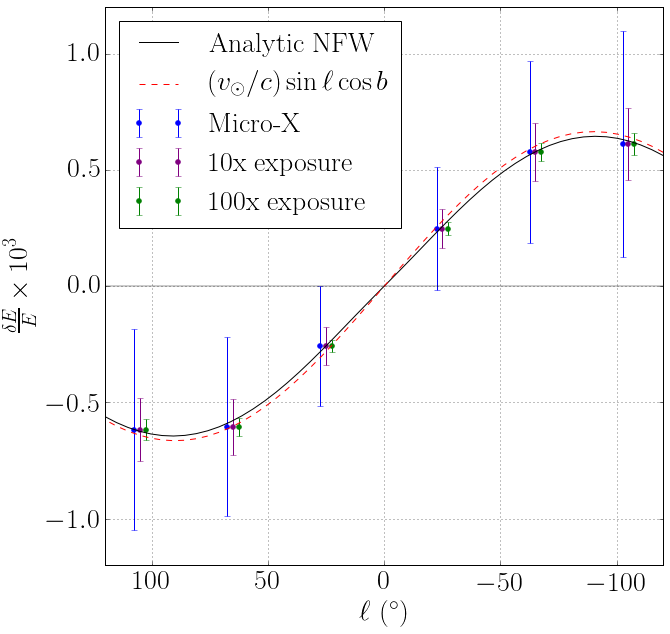
\includegraphics[width=1.0\columnwidth]{de_vs_l.png}
\caption{Velocity spectroscopy on the Milky Way analogue Halo 374. This shows the position of the observed line centroid due to sterile
	neutrino decay as a function of Galactic longitude $\ell$, with latitude $b=25^\circ$.
	Here we compare results as computed from the N-body simulation (see Section \ref{sec:simulations}) for the
	instrumental parameters of Micro-X against our analytic model (Section
	\ref{sec:theory}) as well as a simple sinusoidal model, showing excellent agreement between the
	three. Note that the error bars represent the $1\sigma$ uncertainty
in the energy of the line centroid, given by \eqref{eq:stats}, rather than the Doppler-broadened width of the line.}
\label{fig:de_vs_l}
\end{figure}

%\begin{figure}[h!]
%\centering
%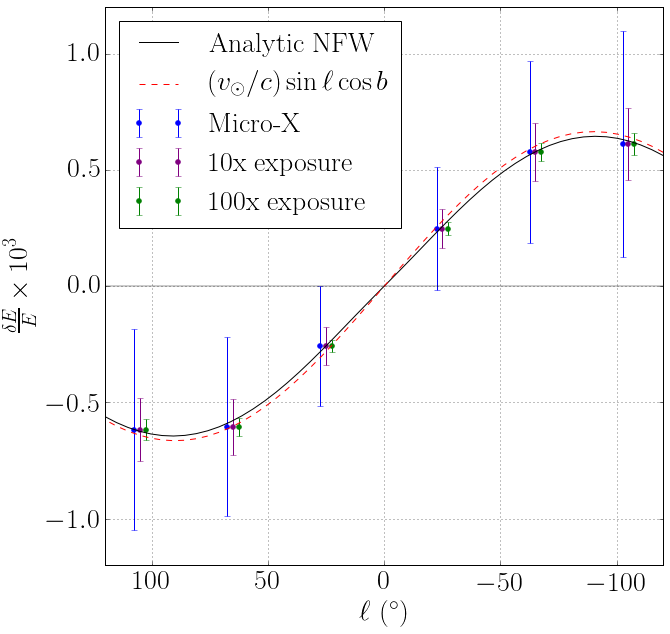
\includegraphics[width=1.0\columnwidth]{de_vs_l.png}
%\caption{Velocity spectroscopy of the Milky Way halo, giving the position of the observed line centroid due to sterile
	%neutrino decay as a function of Galactic longitude $\ell$, with latitude $b=25^\circ$. This
	%compares results as computed from an N-body simulation (Halo 374; see Section \ref{sec:simulations}) for the
	%instrumental parameters of Micro-X against our analytic model (Section
	%\ref{sec:theory}), showing good agreement.	
	%Note that the error bars here represent the 1-$\sigma$ uncertainty
	%in the energy of the line centroid, rather than the Doppler-broadened width of the line.}
%\label{fig:de_vs_l}
%\end{figure}

\begin{figure}[h!]
\centering
\begin{subfigure}[b]{1.0\columnwidth}
	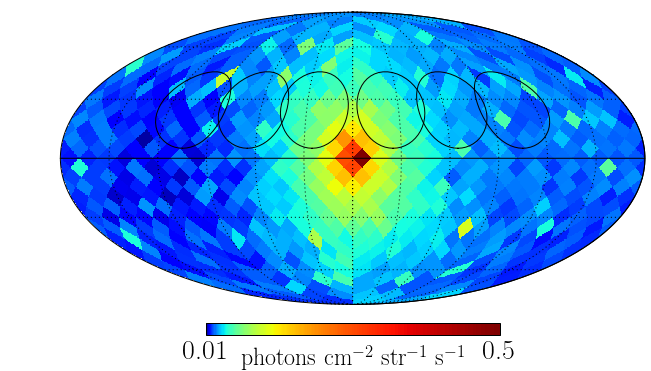
\includegraphics[width=\textwidth]{flux_map_374.png}
\subcaption{Flux.}
\end{subfigure}
\par\medskip
\begin{subfigure}[b]{1.0\columnwidth}
	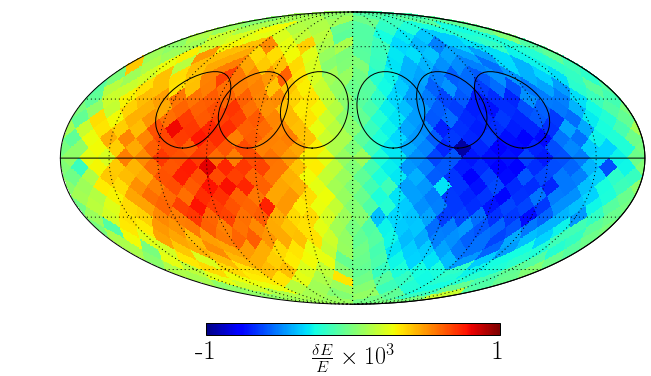
\includegraphics[width=\textwidth]{line_map_374.png}
\subcaption{Doppler-shifted line centroid.}
\end{subfigure}
\par\medskip
\begin{subfigure}[b]{1.0\columnwidth}
	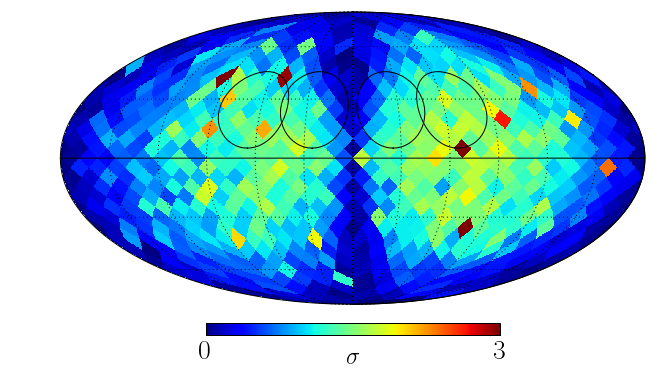
\includegraphics[width=\textwidth]{sigma_map_374.png}
\subcaption{Exclusion of the line centroid from $\delta E/E=0$.}
\end{subfigure}
\caption{Sky maps illustrating the principle of velocity spectroscopy. Top: The flux map. Middle:
	The dipole pattern in the line energy induced by our motion relative to the Milky Way halo.
	Bottom: The signicance of the detection of Doppler shifting of a dark matter decay line,
indicating the number of $\sigma$ by which $\delta E/E=0$ can be excluded for a Micro-X
observation. Black circles indicate the
FOV of Micro-X on the sky for the six pointings used in Figure \ref{fig:de_vs_l}. }
\label{fig:skymaps}
\end{figure}



%\subsection{Halo triaxiality}
%\label{sec:triaxiality}

\begin{figure}[h!]
\centering
\begin{subfigure}[b]{1.0\columnwidth}
	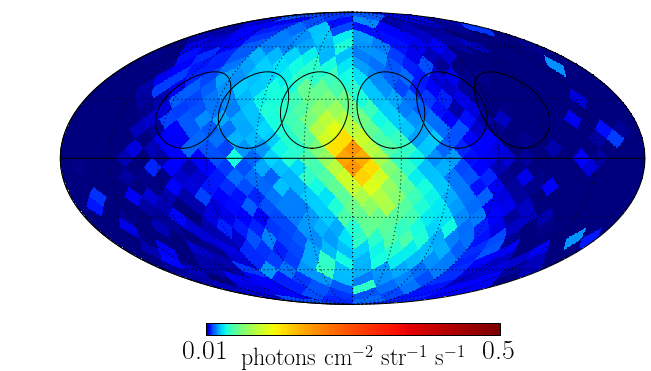
\includegraphics[width=\textwidth]{flux_map_800.png}
\end{subfigure}
\par\medskip
\begin{subfigure}[b]{1.0\columnwidth}
	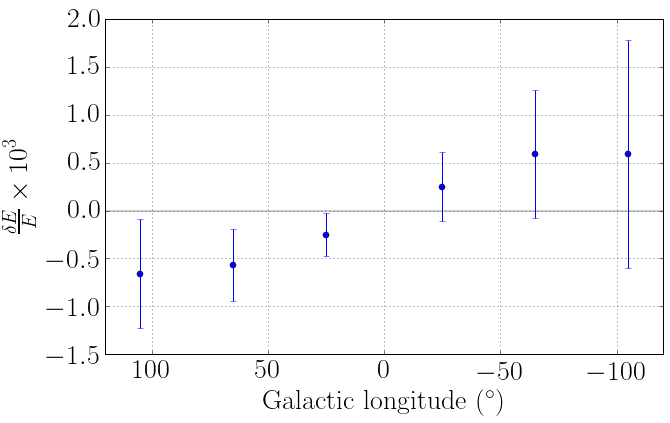
\includegraphics[width=\textwidth]{de_vs_l_800.png}
\end{subfigure}
\caption{Asymmetry of the Milky Way halo (here, Halo 800 with $b/a=$ and $c/a=$) could skew the significance of the
	observed signal to the east or west. Each field of view (black circles in the sky map) corresponds to a data point in
the lower plot. The gray shaded region indicates the $1\sigma$ uncertainties for the analytic model
derived from a spherical NFW profile fit to this halo.}
\label{fig:triax}
\end{figure}




% % % % % % % % % % % CONCLUSIONS % % % % % % % % % % % % % % % % % % % % % %
\section{Conclusions}
\label{sec:conclusions}

Very often in the past, anomalous astrophysical signals have been interpreted as the signature of dark matter.  However, none of these extraordinary claims survived the scrutiny of extraordinary evidence.  All of these false alarms raises an important question:  can we design a new test to confirm the dark matter origin of an anomalous astrophysical signal?  The answer is yes, and Ref.\,\cite{speckhard2016} showed that telescopes with $\mathcal{O}$(0.1\%) energy resolution can utilize the Doppler effect of a sharp signal arising from dark matter interactions to perform dark matter velocity spectroscopy.

We look into this issue in detail in this work.

 
\vspace{-0.5 cm}
	
% % % % % % % % % % % % % % % % % % % % % % % % % % % % % % % % % % % % % %		

% % % % % % % % % % % % % % % %Acknowledgments % % % % % % % % % % % % % % %
\section*{Acknowledgments} 

Mark Lovell, Yao-Yuan Mao, Chris Davis.

% % % % % % % % % % % % % % % % % % % % % % % % % % % % % % % % % % % % % % % % %	

\newcommand{\mnras}[0]{M.N.R.A.S.}
%\bibliographystyle{kp}
%\bibliography{Bibliography/references}	
\bibliography{references}	

\end{document}
